\subsection{Report}\label{sec:ecg:report}
The main goal of this project is to build a basic ECG arrhythmia detetection model. We are using a ECG dataset we pulled from PhysioNet. However before we can do that properly with the provided data our first task at hand was to process/filter the signals, through Identifying QRS Complexs (R-Peaks) and the corresponding features such as RR Intervals.
\\
\\
To begin, we installed and configured the following Python packages:
\begin{itemize}
    \item \texttt{numpy} – Various mathematical operations and processing
    \item \texttt{scipy} – filtering and reading '.mat' files
    \item \texttt{matplotlib} – Signal Visualization
    \item \texttt{py-ecg-detectors}  - Useful algorithims to aid in identifying QRS Complexes and RR Intervals
\end{itemize}

\subsection{Milestones}\label{sec:ecg:milestones}
We implemented code that recursively processes `.mat` ECG files. It does so by applying a filter to the signal and then downsmapling it to reduce the overall noise/complexity. Then it visualizes the processed waveform and detects R-Peaks with a Pan-Tompkins Algorithim. Also RR intervals are computed and summarized for each recording for future use.

Some major components of the implementation included:
\begin{itemize}
    \item Preprocessing/Filtering ECG signals with low-pass Butterworth filtering
    \item Downsampling to reduce noise and improve performance of the signals
    \item Visualizing filtered ECG signals with time-domain plots
    \item Extracting useful information in such as RR Intervals
\end{itemize}

\begin{figure}
	\centering
	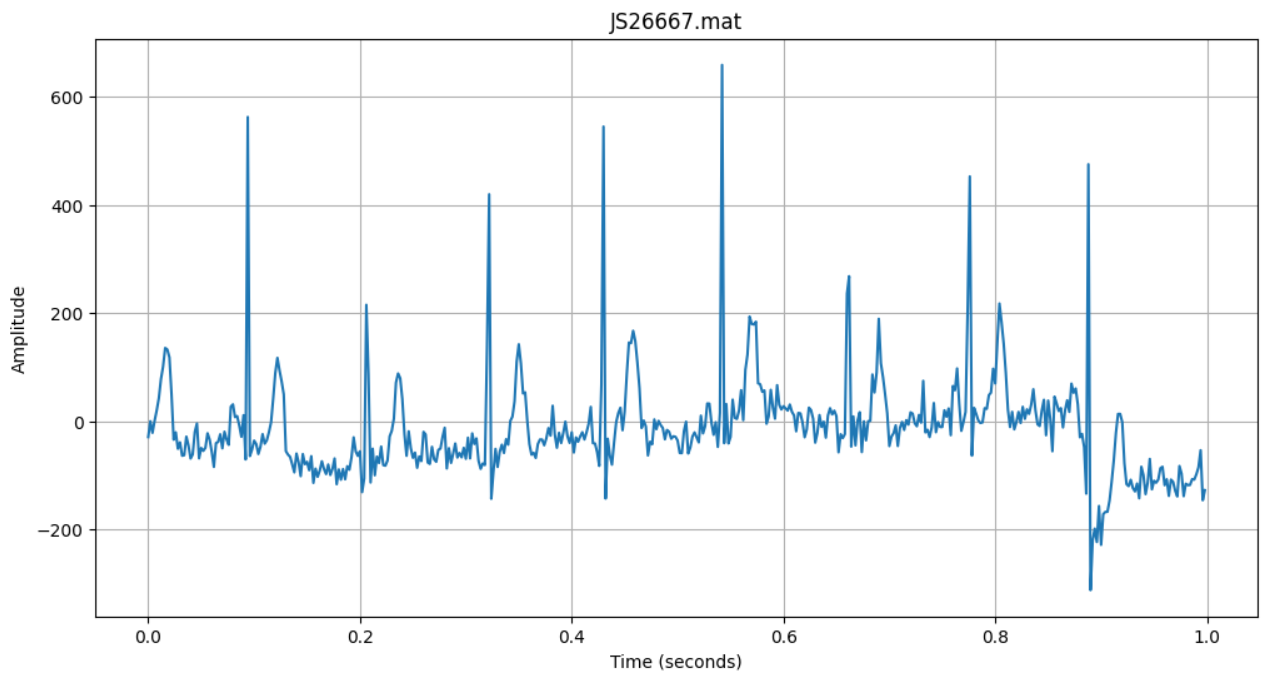
\includegraphics[width=15cm]{signal}
	\caption{Sample of a Processed ECG signal}
	\label{fig:Signal}
\end{figure}

\subsection{Important Links}\label{sec:ecg:links}
\begin{itemize}
    \item \textbf{\texttt{py-ecg-detectors} Documentation}: \href{https://pypi.org/project/py-ecg-detectors/}{https://pypi.org/project/py-ecg-detectors/}
    \item \textbf{Dataset}: \href{https://physionet.org/content/}{https://physionet.org/content/}
    \item \textbf{Guide we used for ECG Filtering}: \href{https://medium.com/@shahbaz.gondal588/understanding-ecg-signal-processing-with-python-b9dd4ea68682}{https://medium.com/@shahbaz.gondal588/understanding-ecg-signal-processing-with-python-b9dd4ea68682}
\end{itemize}
